\documentclass[a4paper,12pt]{article}
\usepackage[utf8]{inputenc}
\usepackage[slovak]{babel}
\usepackage{hyperref}
\usepackage{graphicx}
\usepackage{fancyhdr}
\usepackage{titlesec}

\usepackage{listings}
\usepackage{csquotes}
\usepackage{dirtree}


% Nastavenie titulnej strany
\begin{document}

\begin{titlepage}
    \centering
    \vspace*{1cm}
    \Large{\textbf{Technická univerzita v Košiciach}\\
    Fakulta elektrotechniky a informatiky}\\
    \vfill
    \large{Formálne jazyky}\\
    \large{Dokumentácia k obhajobe zadania}
    \vfill
    \begin{flushleft}
        Oleniuk Vladyslav\\
        Akademický rok: 2024/2025\\
        Študijný program: Informatika
    \end{flushleft}
\end{titlepage}

\tableofcontents
\newpage

\section{Formulácia zadania}


Cieľom zadania je implementovať jednoduchý generátor konečnostavových automatov (NKA) zo zadaného regulárneho výrazu využitím metódy jeho syntaktickej analýzy zhora nadol rekurzívnym zostupom.

\subsection{Vstup}

Na vstupe sa očakáva ľubovoľný reťazec znakov reprezentujúci regulárny výraz v na tomto predmete štandardne využívanej notácii.

\subsection{Výstup}

Program bude mať nasledujúce výstupy:
\begin{itemize}
    \item grafická reprezentácia stromu odvodenia pre zadaný regulárny výraz,
    \item plne funkčná programová implementácia nedeterministického konečnostavového akceptora zodpovedajúceho zadanému regulárnemu výrazu.
\end{itemize}

\section{Vypracovanie zadania}

Zadanie bolo vypracované v jazyku python.

\subsection{Opis architektúry riešenia}
Všeobecná štruktúra programu je nasledovná:
\dirtree{%
    .1 src/.
    .2 Lexer.py.
    .2 Parser.py.
    .2 main.py.
    .2 (nka.py).
}
\subsubsection{Lexer.py}
Lexer.py rozdeľuje vstupný reťazec na lexémy a zakóduje ich do tokenov.
Vytvoril som nasledujúce typy tokenov:
\lstset{basicstyle=\ttfamily}
\begin{lstlisting}
SYMBOL -> akykolvek iny symbol okrem nizsie uvedenych
LPAREN -> (
RPAREN -> )
LCBRA  -> {
RCBRA  -> }
LBRACK -> [
RBRACK -> ]
PIPE   -> |
EOF    -> koniec vstupu
\end{lstlisting}

\subsubsection{Parser.py}
Súbor Parser.py slúži na syntaktickú analýzu, pričom využíva techniku rekurzívneho zostupu.
Počas analýzy konštruuje strom odvodenia.

\subsubsection{main.py}
Hlavný súbor aplikácie, prostredníctvom ktorého sa spúšťa.
Zároveň vykonáva zápis výsledného NKA do súboru \textit{nka.py}.

\subsection{Gramatika jazyka regulárnych výrazov}

\lstset{basicstyle=\ttfamily}
\begin{lstlisting}
    regular ::= 'eps' | alternative
alternative ::= sequence {'|' sequence}
   sequence ::= element {element}
    element ::= symbol | '(' alternative ')' | '[' alternative ']' | '{' alternative '}'

\end{lstlisting}

\subsection{Podrobný postup implementácie}

% Detailný popis implementácie

\subsection{Ukážka vstupu a prezentácia výsledkov}

\begin{figure}
    \centering
    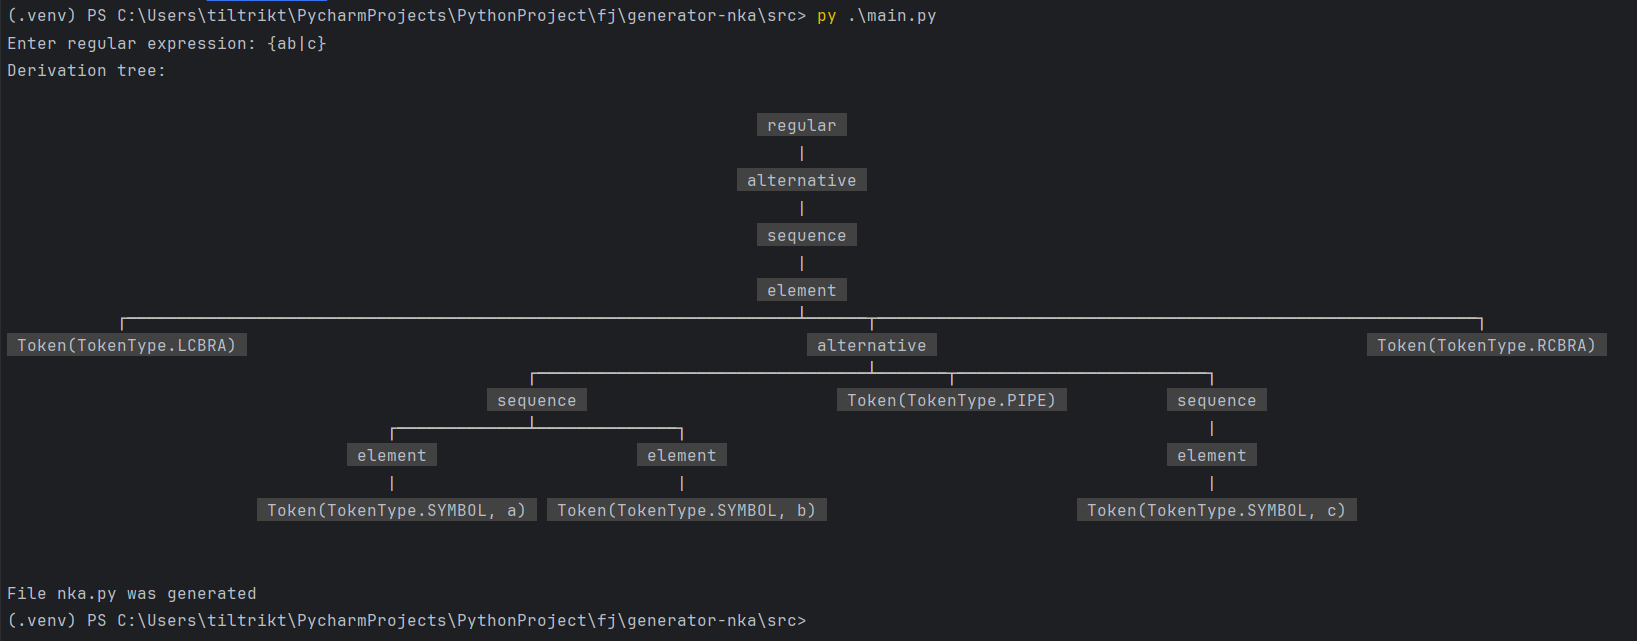
\includegraphics[width=1\textwidth]{figs/tree-example}
    \caption{Príklad vstupu}
    \label{fig:tree-example}
\end{figure}
Po spustení programu sa vygeneruje strom zobrazený na obrázku~\ref{fig:tree-example} a súbor \textit{nka.py}.
Vygenerovaný súbor \textit{nka.py} funguje nasledovne:
\lstset{basicstyle=\ttfamily}
\begin{lstlisting}
(.venv) PS ...\generator-nka\src> py .\nka.py
Enter a word:
Word '' is ACCEPTED!
Enter a word: ab
Word 'ab' is ACCEPTED!
Enter a word: c
Word 'c' is ACCEPTED!
Enter a word: ababcccabc
Word 'ababcccabc' is ACCEPTED!
Enter a word: acb
Word 'acb' is NOT ACCEPTED!
Enter a word: ab123
Word 'ab123' is NOT ACCEPTED!
Enter a word: quit
(.venv) PS ...\generator-nka\src>
\end{lstlisting}


\subsection{Problémy a ich riešenie}

Dlho som nevedel prísť na to, ako vytvoriť tabuľku prechodov.
Po nejakom čase som si prezrel webovú stránku \href{https://kurzy.kpi.fei.tuke.sk/fj/}{Formálne jazyky} a našiel som Thompsonovu konštrukciu.
Po niekoľkých neúspešných pokusoch sa mi podarilo implementovať generovanie tabuľky pre jednoduchý regulárny výraz \textit{ab}, a tak som sa rozhodol pokračovať v postupe týmto smerom.


\subsection{Hodnotenie zadania}

Úloha bola veľmi zaujímavá a pomohla mi lepšie pochopiť mnohé témy. Jediným problémom, s ktorým som sa stretol, bolo nájsť knižnicu na nakreslenie stromu. Ušetril by som veľa času, keby bolo niekoľko poskytnutých v samotnom zadaní.

\section{Vyhodnotenie a záver}

Podarilo sa mi implementovať všetko. Úloha sa testovala na niekoľkých rôznych vstupoch: správnych, nesprávnych a prázdnych. Nemusel som sa zaseknúť na žiadnom bode na dlhší čas.

\end{document}